\documentclass{article}
\usepackage[utf8]{inputenc}
\usepackage{amsmath}
\usepackage{amssymb}
\usepackage{changepage}
\usepackage{graphicx}
\allowdisplaybreaks
\title{Homework 3b Writeup}
\author{Michael Tang}
\date{due May 21, 2019}
\begin{document}
\maketitle
\begin{adjustwidth}{-2cm}{-2cm}
\section{Usage}
Use ``make'' to compile and link the modules from utils and from the root directory. ``make clean'' is available to remove all .o files.\\
Execute the program as follows:\\
./pacver [-n \textit{nthreads}] [-W \textit{pkwk}][-M \textit{timelim}][-T \textit{npck}][-D \textit{qdepth}][-u \textit{uniflag}][-x \textit{rngseed}][-p \textit{pflag}][-S \textit{opmode}][-L \textit{lockmode}][-o \textit{outpath}]
\begin{itemize}
	\item -n specifies number of sources. In parallel mode this translates to number of worker threads (so the total number of threads will be n+1). Required.
	\item -W specifies average work per packet. Required.
	\item -M specifies time limit for threads, in milliseconds. All threads will run until the time limit is reached. Due to time difference measurement in-program being based in seconds, -M must be a multiple of 1000. Either this or -T but \textbf{not both} must be specified.
	\item -T specifies number of packets each worker thread is to process. This was used for correctness testing purposes only. This XOR -M must be specified.
	\item -D specifies queue depth, default 8 if not specified.
	\item -u is a flag that has default value 1. If 0, packets will follow exponential load distribution, if 1, packets will follow uniform load distribution.
	\item -x specifies the seed for the packet generator. For all tests, -x 23 was used. Required.
	\item -p is a flag with default value 0. If 0, the program will run in serial mode, if 1, the program will run in parallel mode.
	\item -S specifies the strategy to use in parallel mode, with 0-2 being LockFree, HomeQueue, and Awesome modes in sequence. Required if -p 1, ignored if -p 0.
	\item -L specifies lock type, 0-3 for TASLock, PThread\_Mutex, ALock, and CLHLock in sequence. Required if -p 1 and -S > 0 is specified.
	\item -o is the path for the file to which user wants to output. If not specified, program will default to stdout. \textbf{WARNING:} files open in append mode. If you want to start a clean version of existing output files make sure to remove them first.
\end{itemize} 

\section{Design Changes}
\subsection{Input, Initialization, and Output}
Following clarification in design review of how we were supposed to use -T and -M, both arguments have been supported. -u and -p were added to provide additional operation detail.\\
Operation flow remains the same as specified in the design document, and as in HW2: from argument parsing in main() to thread preparation and launch in opcontrol(), with the dispatcher thread calling dispatcher() and the worker threads calling operator().\\
Relevant outputs - specifically total packets dispatched, packets checked per thread, total packets checked, and sum of checksums - have been moved to post-operation of all threads instead of in the middle of operation. I.e., instead of printing checksums as they process them, worker threads now add the checksum to a running thread subtotal, then write that subtotal to their private slot in an array that holds all thread subtotals. All those subtotals are added up to get the total sum of checksums, which is printed at the end of opcontrol(). This significantly saves critical section operation time and allows the program to have higher throughput.
\subsection{Queue Attachment Strategy}
The design is more fleshed out here than in the design document. The operator() function measures time from the beginning of actual operation (trying deq() for LockFree, trying to grab the queue's lock for HomeQueue, and trying to find a free queue for Awesome), then jumps to output information writing and termination after that time limit is reached. Difference from start time is measured with the <time.h> function difftime().\\
LockFree operation remains the same as in HW2. HomeQueue first grabs the home queue's lock with TryLock, then performs the same operation as LockFree. After deq() and checksum are finished on the packet, the thread releases the lock and starts from the top of the operation loop.\\
Awesome mode has each thread start with the queue that they would be attached to in HomeQueue/LockFree, and like in HomeQueue they grab that queue's lock. However, if either TryLock returns that the lock is busy or deq() returns that the queue is empty, the thread will begin iterating over all queues until it can find one that has an open lock AND is not empty. Importantly, after a packet is successfully dequeued the thread releases that queue's lock. This allows other threads to begin pulling other packets even while the first thread is still checksumming. Admittedly this placement of unlock() could also have been done for LockFree, but it makes no difference there because it is only one thread that will ever operate on that queue.

\section{Testing Results}
\subsection{Correctness}
I followed through with my decision in the design document to not test the locks or Lamport queue in-depth for any of their invariants, because they have already been tested and proven correct in Homeworks 3a and 2 respectively. However, just to be sure, I set up tests with a fixed number of packets per queue -T across all modes to test the non-dropping and correct processing invariants. These tests output number of packets dispatched as well as total number of packets processed, and the total sum of checksums. For the program to be correct, the number of packets dispatched must equal the total number of packets processed each session (to ensure non-dropping) and the total sum of checksums must be the same as serial mode across all modes. For the sum of checksums comparison, uniform sessions were compared with serial-uniform, and exponential sessions were compared with serial-exponential. The output (3b\_tests/actual\_correctness.txt, outputted from the CSIL Linux machine with shell script /3b\_tests/corrcommands) was then run through a Python 3 script (3b\_tests/correctness\_check.py), which outputs any incorrectnesses to 3b\_tests/correctness\_ver.txt.\\
There were no discrepancies discovered, so we can safely conclude that the program runs correctly.

\subsection{Performance}
All performance tests were performed as directed in the instructions; Awesome Mode tests will be detailed in their section. All trials of all modes in every experiment was repeated 5 times and the statistic averaged across those 5 trials. -M 2000 was picked because trials were observed to have little variance while keeping the runtime of experiments from being too high.\\
All performance test outputs are available in hw3/3b\_tests, and data was put through Jupyter notebooks using Python 3 and the Pandas package to output the needed data tables. The notebooks can also be found in 3b\_tests and are labelled according to their experiment. 
\subsubsection{Idle Lock Overhead}
First is the measurement of lock overhead via comparison of HomeQueue throughputs to LockFree. The data and graph for this are below.\\
\null\\
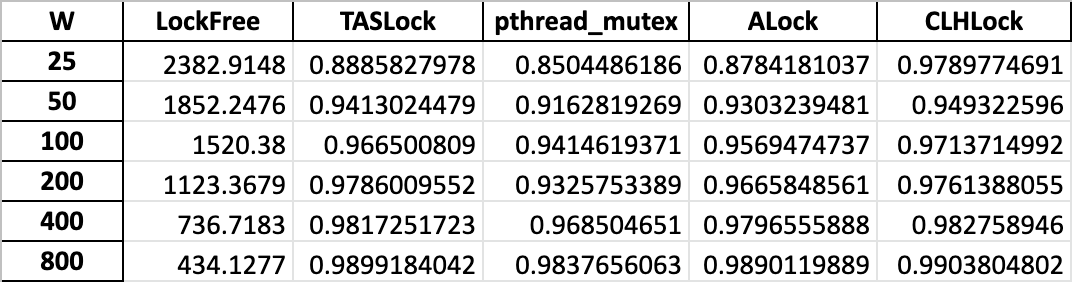
\includegraphics[width=\linewidth]{b_overhead2freeData.png}\\ \null\\
\null\\
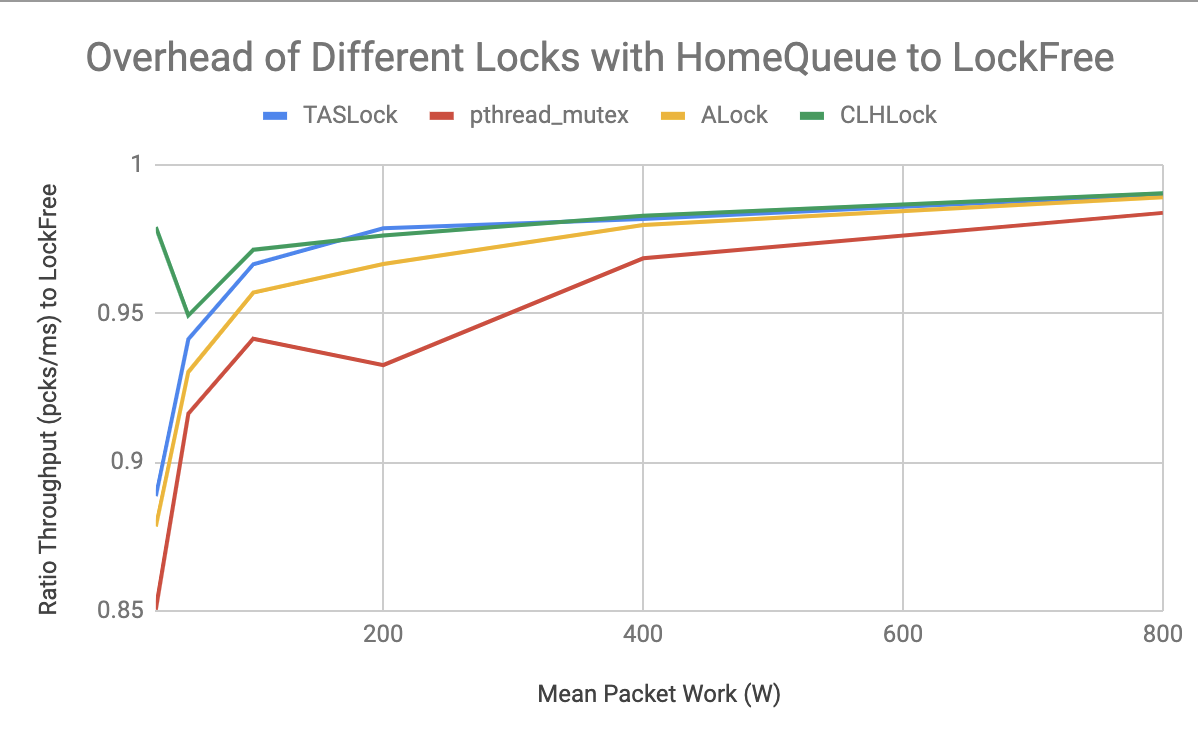
\includegraphics[width=\linewidth]{b_overhead2freeGraph.png}\\ \null\\
Contrary to my hypothesis in the design document but in agreement with the results of the lock overhead testing for Part a, HomeQueue across all locks increased in speed as $W$ increased, converging to a speedup ratio of about .99. At all $W$ levels CLHLock, TASLock and ALock had higher throughput levels than pthread\_mutex, with TASLock and CLHLock having neck and neck performance while ALock, initially lagging TASLock by .01 (in speedup ratio), caught up to only lag TASLock by .0009. This too is consistent with Part (a) overhead testing.\\
I hypothesize again that ALock is slower than CLHLock because both have the same queue creation overhead but the getAndIncrement() call that ALock uses to change its tail pointer is slower than the testAndSet() call that CLHLock uses for the same.\\
\null\\Below are the data and graph for comparison of worker rates to the serial-queue results of HW2.\\
\null\\
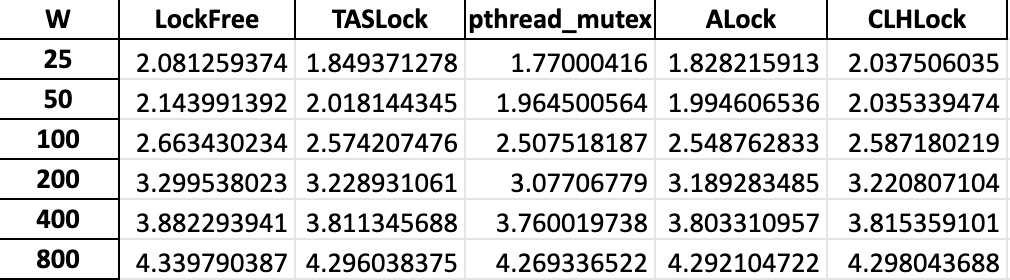
\includegraphics[width=\linewidth]{b_overhead2sqData.png}\\ \null\\
\null\\
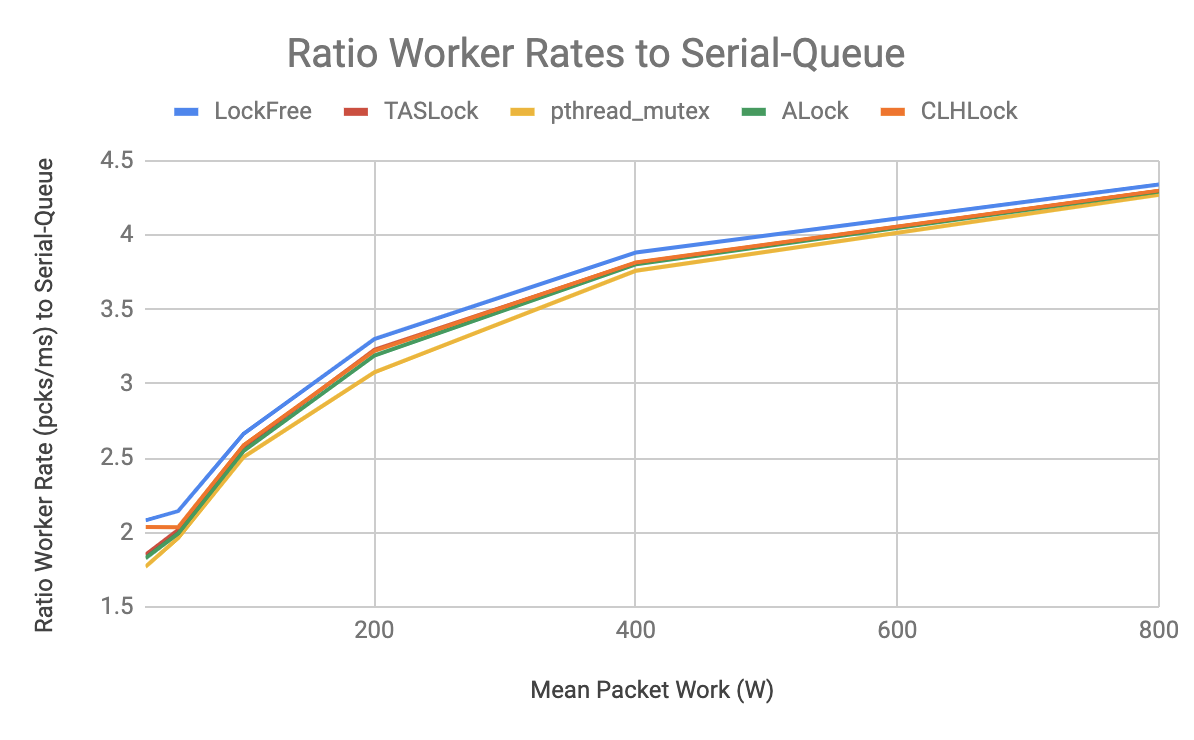
\includegraphics[width=\linewidth]{b_overhead2sqGraph.png}\\ \null\\
All modes experienced a higher worker rate than serial-queue, starting at around $2\times$ at $W=25$ and ending as high as $4.33\times$ at $W=800$. As is expected due to overhead, all HomeQueue modes had a smaller worker rate increase than LockFree. Between the HomeQueue modes worker rate increase was fairly equivalent, with TASLock maintaining the highest throughout except for $W=800$, where pthread\_mutex was highest. This is due to the fact that one lock is only ever accessed by one thread, making contention a non-issue and removing the worker rate advantages related to contention for ALock and CLHLock.

\subsubsection{Speedup with Uniform Load}
First below are the data and graph for speedup of LockFree and HomeQueue with various locks to serial with a uniform load, at average packet work of 1000 ($W = 1000$).\\
\null\\
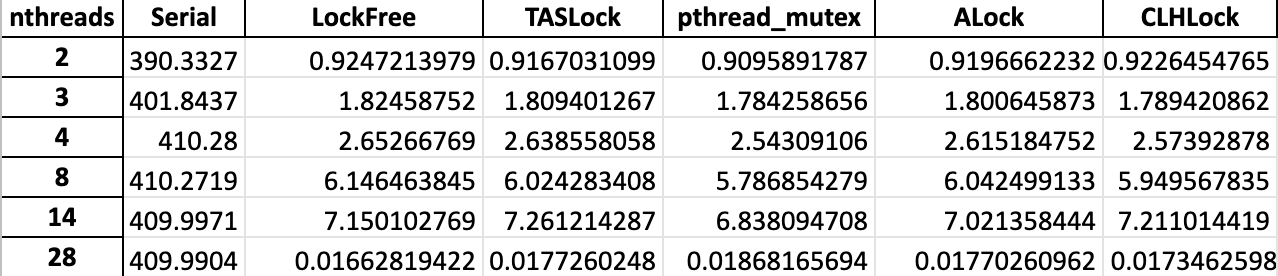
\includegraphics[width=\linewidth]{b_uni1000Data.png}\\ \null\\
\null\\
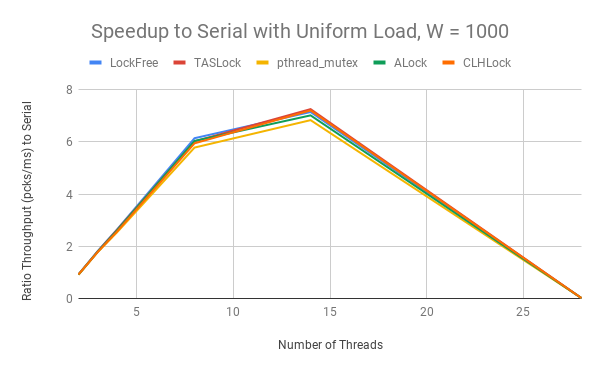
\includegraphics[width=\linewidth]{b_uni1000Graph.png}\\ \null\\
In line with expectations, LockFree performed the same as in Homework 2.\\
All parallel modes followed approximately the same throughput speedup, going from around $0.9\times$ serial at 2 sources to $7\times$ serial at 14 threads, back down to $0.02\times$ serial at 28 threads. The collapse in speedup from 14 to 28 threads can be explained by the fact that SLURM only has 14 nodes usable by testers - beyond that, multiple threads can populate one core and context switching between threads of the same core ruins parallelism.\\
Mostly following expectations of lock overhead, LockFree performs better than all the lock modes except at 14 and 28 threads. At 14 threads, LockFree is outperformed by TASLock and CLHLock, and at 28 threads all versions of HomeQueue outperform LockFree.\\
At 28 threads, the difference between all the parallel modes is at its smallest, and there could likely have been larger relative variances in throughput between trials depending on how the SLURM cluster handled context switching during that session. So I venture to say that at that point the parallel modes can be regarded as approximately equal, with many more trials needed to even out variance if we want to more granularly distinguish them.\\
However, the better performance of TASLock and CLHLock at 14 threads is on a wider margin, and there is no inter-thread context switching at that many threads. This defies my expectations and also goes against the insights of the Idle Lock Overhead experiment. The only two explanations I can think of are that the additional delay added with lock handling reduced the necessary memory barrier synchronization delay, or that at that specific number of threads the variance was too high for 5 trials to even it out. Future experimentation would extend the -M runtime limit to figure out which of those two explanations are more valid.\\
What did follow my initial hypothesis, though, was that speedup rankings of the HomeQueue modes generally went in the order (from fastest to slowest) observed in Part (a) overhead testing and the Idle Lock Overhead test above: TASLock, CLHLock, ALock, pthread\_mutex.\\
\null\\Next are the data and graph for the same speedup experiment but with $W=2000$.\\
\null\\
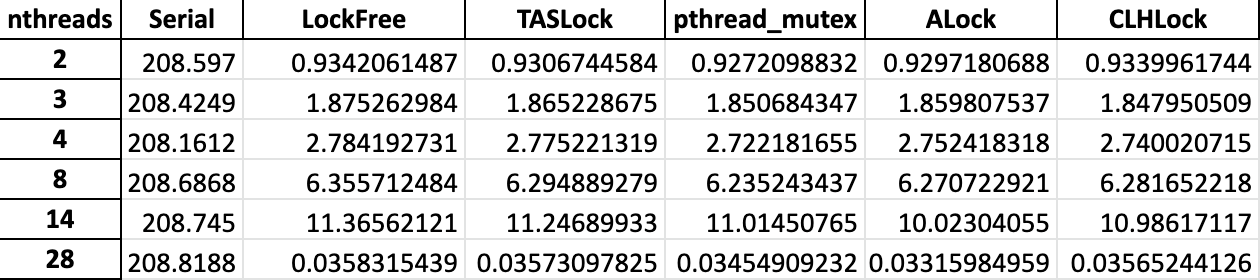
\includegraphics[width=\linewidth]{b_uni2000Data.png}\\ \null\\
\null\\
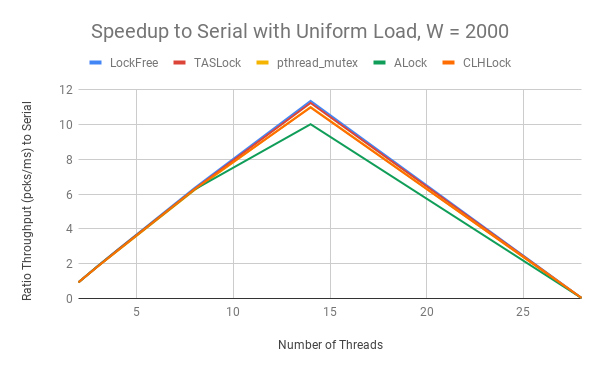
\includegraphics[width=\linewidth]{b_uni2000Graph.png}\\ \null\\
Following my expectations before testing, the speedup of all LockFree and HomeQueue modes over serial mode improved substantially with this jump in $W$. This can be attributed to dispatch throughput in serial mode being dependent on processing throughput, since serial mode alternates between dispatch and processing on one thread. Parallel modes, with their dispatch speed independent of processing speed, would not experience the full effects of this bottleneck. The numbers back this up - in this case, at 14 threads serial mode experienced a 49.1\% decrease in throughput from $W=1000$ to $W=2000$ - approximately halving it, inversely proportional to the doubling of $W$. LockFree and HomeQueue modes, on the other hand, only experienced approximately a 20\% average decrease at the same number of threads and with the same change of $W$.\\
What was not predicted beforehand was the slowdown of ALock and CLHLock relative to pthread\_mutex, especially the substantial relative slowdown of ALock. The only thing that has changed regarding the locks are distance from lock acquisition to lock release in a single attempted dequeue. Based off of this, I extend the tenuous explanation that the address of a thread's slot in the queue, which is stored as part of the lock structure for my implementation of both queue-based locks, was cached during lock(), but for longer periods between lock operation (longer work time for packet from larger $W$) that cache line may have been more likely to be removed before unlock() was called, by another context on the same core. Thus, upon calling unlock() and not having the slot address readily available on cache, the thread would have to read from memory. The additional $W$ may have made this time cost, which pthread\_mutex does not have, more significant than the time benefit that ALock and CLHLock have of not using system calls.\\
\null\\Next are the data and graph for $W=4000$.\\
\null\\
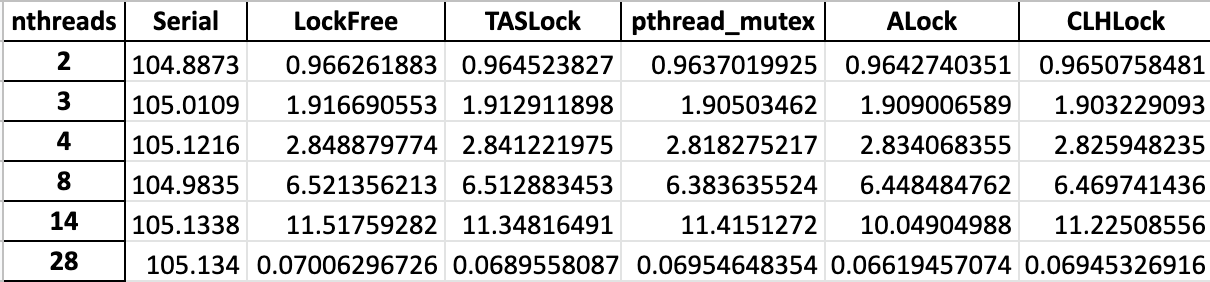
\includegraphics[width=\linewidth]{b_uni4000Data.png}\\ \null\\
\null\\
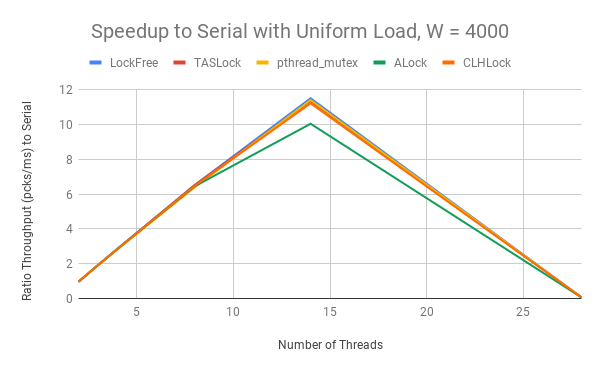
\includegraphics[width=\linewidth]{b_uni4000Graph.png}\\ \null\\
Here pretty much the same picture is given as for $W=2000$, meaning the speedup ratios themselves are approximately the same and the relative ordering of speedup ratios is also the same. The lack of change in ratios to serial but the continued inversely proportional decrease of serial throughput means that this inverse proportion of throughput to work is also now applicable to LockFree and HomeQueue. This goes against my expectations prior to testing, and the best explanation for this happening is that the work bottleneck, while continuing to only exist on worker threads, is now large enough to become a direct bottleneck for the entire process.\\
\null\\Last are the data and graph for $W=8000$.\\
\null\\
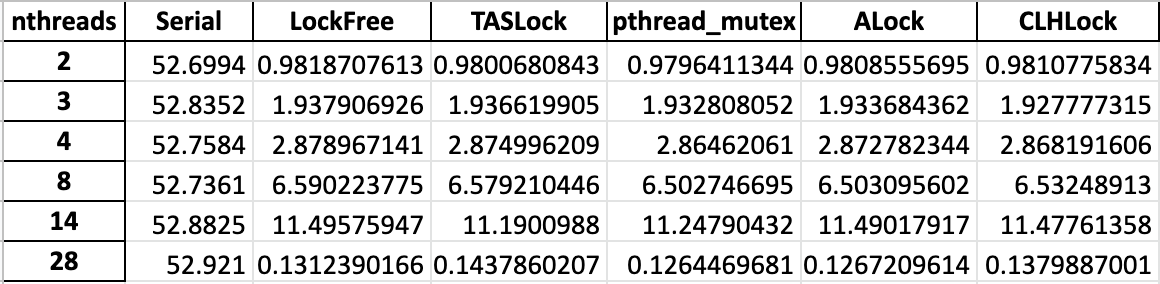
\includegraphics[width=\linewidth]{b_uni8000Data.png}\\ \null\\
\null\\
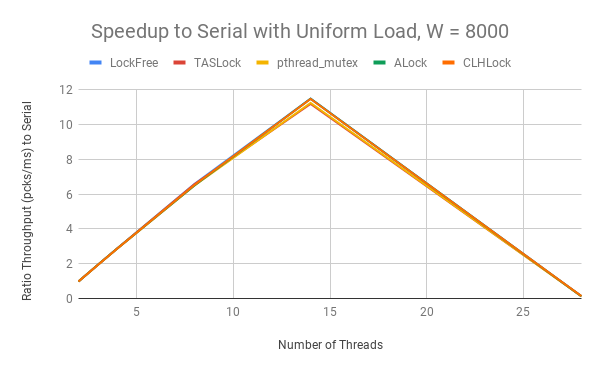
\includegraphics[width=\linewidth]{b_uni8000Graph.png}\\ \null\\
The ratios to serial remain approximately the same, following my explanation for the $W=4000$ data of $W$ becoming a direct bottleneck on the parallel modes at higher amounts.\\
However, ALock and CLHLock are now faster than pthread\_mutex, and TASLock becomes the slowest at 14 threads. To keep in line with my explanations of why the queue-based locks were relatively slower than pthread\_mutex at $W=(2000,4000)$, I can only say that at $W=8000$, these differences no longer matter as the time taken to work on the packet is long enough to dwarf any lock-based overhead.\\
To support this, note that LockFree, while still being relatively faster than the HomeQueue modes, is much less so at this $W$, and is even outpaced by TASLock and CLHLock at 28 threads.

\subsubsection{Speedup with Exponential Load}
First below are the data and graph for speedup of LockFree and HomeQueue with various locks to serial with an exponential load, at average packet work of 1000 ($W = 1000$).\\
\null\\
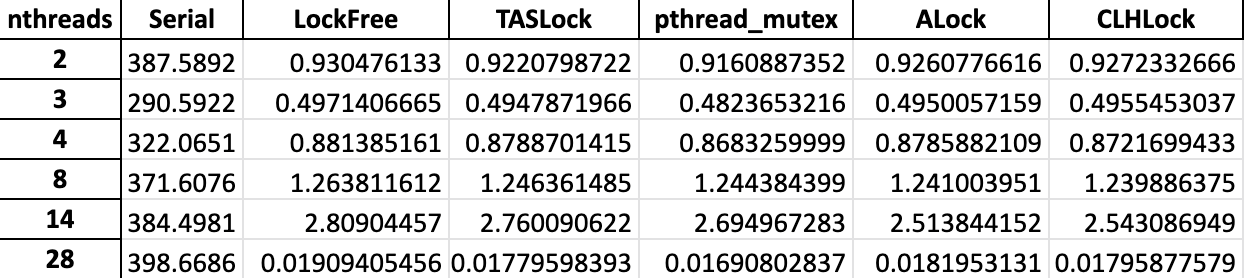
\includegraphics[width=\linewidth]{b_exp1000Data.png}\\ \null\\
\null\\
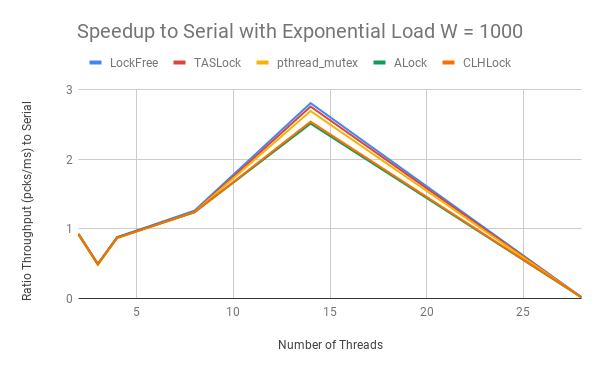
\includegraphics[width=\linewidth]{b_exp1000Graph.png}\\ \null\\
LockFree here performed the same as in Homework 2. Like in Homework 2, this speedup over serial is substantially lower than with uniform load - at 14 threads, LockFree is 60.7\% slower at $W=1000$ with exponential load than with uniform load. Also following expectations is that up until a certain number of threads (which here is 8), the parallel modes are actually slower than serial mode due to parallelization benefits being crippled by a bigger proportion of threads having unequal loads. Serial mode also takes a throughput dip at those lower source amounts due to a higher proportion of packets being larger load.\\
The HomeQueue modes were again slower than LockFree. However, pthread\_mutex being faster than ALock and CLHLock at 8 threads and above was not hypothesized - this could be due to the same change of significances of different types of overheads that we observed with uniform load at $W=(2000,4000)$.\\
\null\\Next are the data and graph for the same modes and exponential load distribution with $W=2000$.\\
\null\\
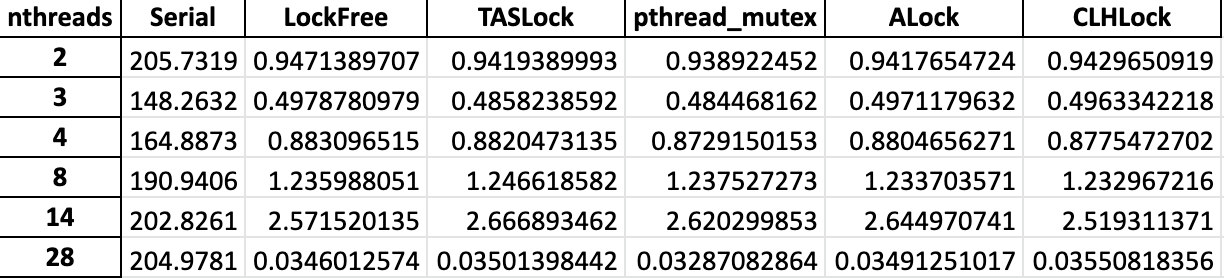
\includegraphics[width=\linewidth]{b_exp2000Data.png}\\ \null\\
\null\\
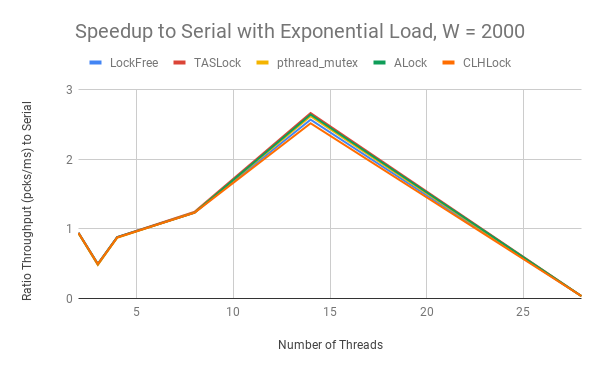
\includegraphics[width=\linewidth]{b_exp2000Graph.png}\\ \null\\
Pretty much the same ratio numbers remain, with the closing of the speedup deficiency of the queue-based locks relative to the other two locks supporting the idea of relative overhead changes that I posited above in exponential, $W=1000$ and in uniform, $W=(2000,4000)$. Absolute throughput of all modes also decreases in inverse proportion to mean work increase, which is as expected because the actual mean work experienced in an exponential load session should be close to the mean work specified.\\
\null\\Next are the data and graph for $W=4000$.\\
\null\\
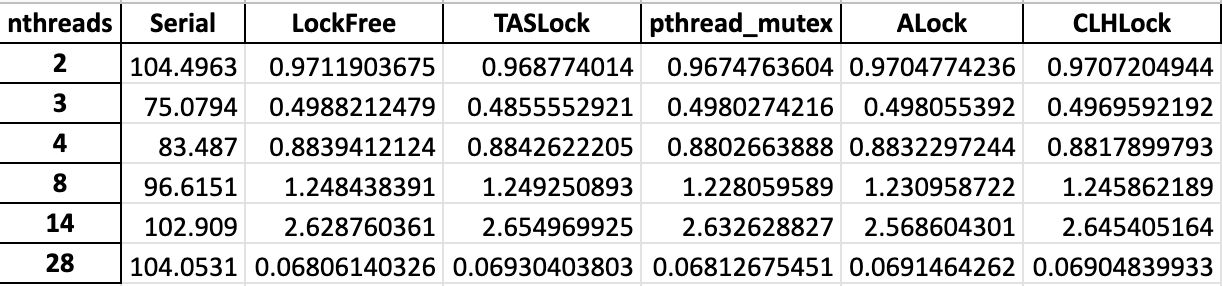
\includegraphics[width=\linewidth]{b_exp4000Data.png}\\ \null\\
\null\\
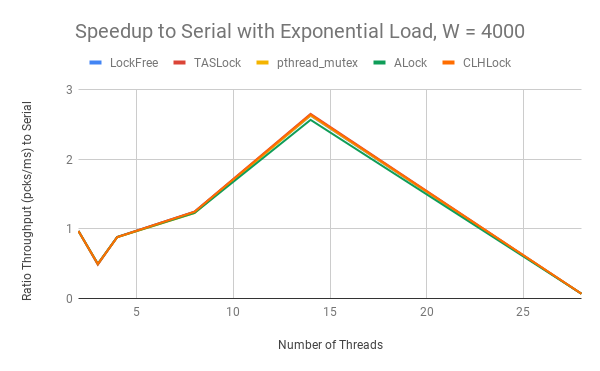
\includegraphics[width=\linewidth]{b_exp4000Graph.png}\\ \null\\
The same ratios remain and the absolute throughput decreases in the same proportion to work increase as before, as expected. Mean work increase has closed the gaps between parallel locks even more, also as expected.\\
\null\\Last are the data and graph for $W=8000$.\\
\null\\
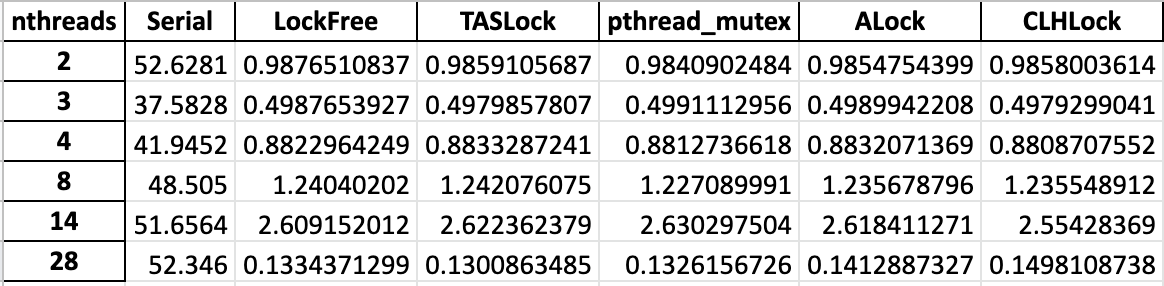
\includegraphics[width=\linewidth]{b_exp8000Data.png}\\ \null\\
\null\\
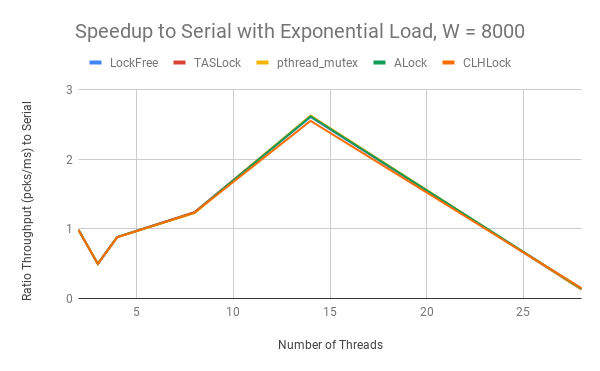
\includegraphics[width=\linewidth]{b_exp8000Graph.png}\\ \null\\
Again the same ratios remain and the throughput decrease is as expected, and the gap between modes has closed so much that they are mostly indistinguishable on the line graph.

\subsubsection{Speedup in Awesome Mode, with Exponential Load}
My implementation of Awesome Mode has the most ideal improvement over the one-thread-one-queue modes when loads are unbalanced between queues. In this case it would be best for threads with less work to transition to processing queues with more work when their own queue is empty. So, I conducted the exponential speedup experiment again but this time with LockFree and Awesome Mode with all of the locks.\\
I expected that LockFree would be an adequate comparison measure instead of having to also add data for HomeQueue sessions, because throughput for LockFree and HomeQueue would be fairly close. The results of the HomeQueue with exponential load experiment vindicate this.\\
\null\\First below are the data and graph for speedup of LockFree and Awesome with various locks to serial with an exponential load, at $W=1000$.\\
\null\\
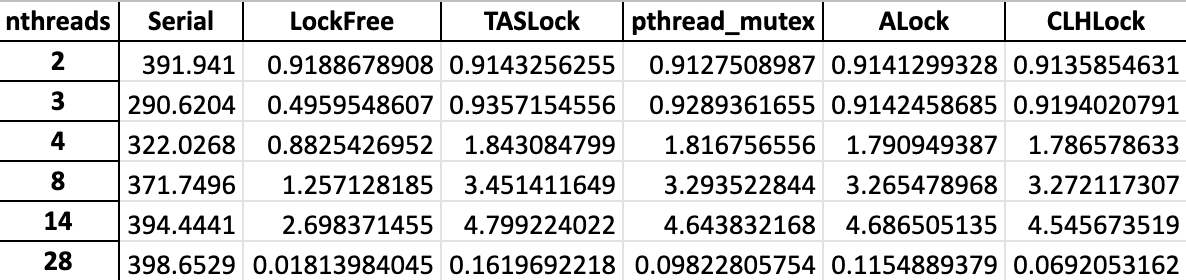
\includegraphics[width=\linewidth]{b_awe1000Data.png}\\ \null\\
\null\\
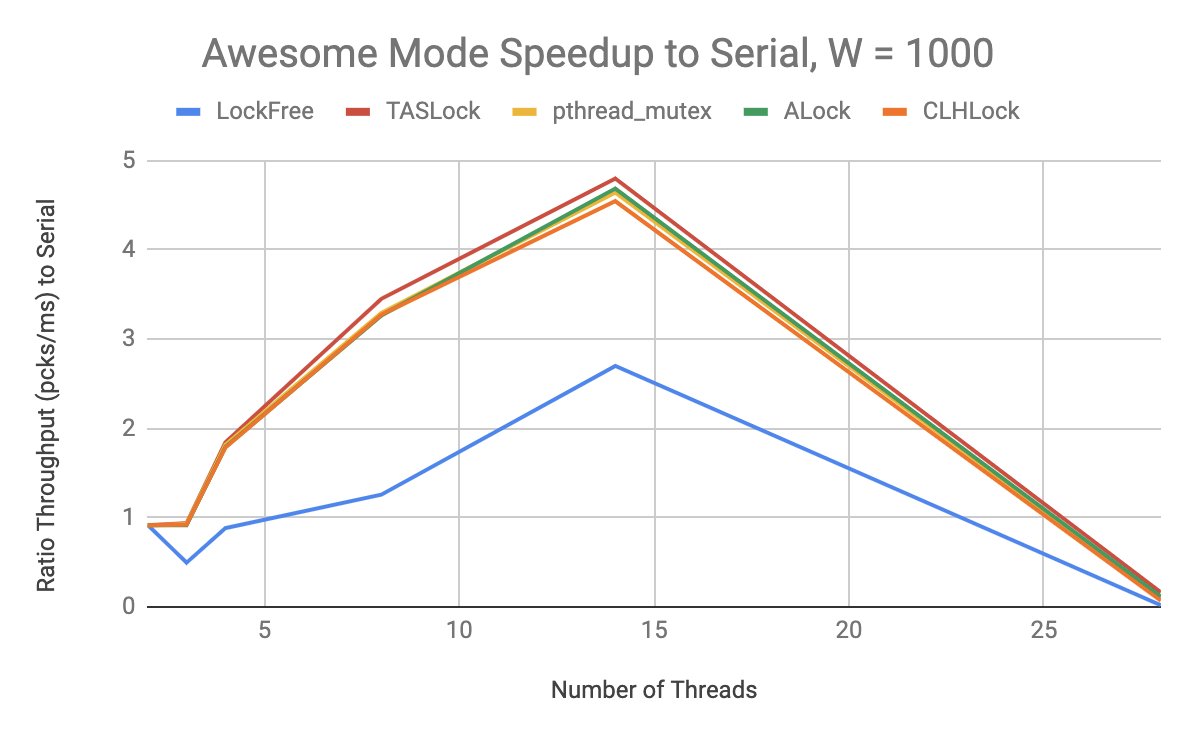
\includegraphics[width=\linewidth]{b_awe1000Graph.png}\\ \null\\
Immediately noticeable and as hypothesized is a significant jump in throughput from LockFree to Awesome. Specifically, at 14 threads, the best performing lock TASLock was $1.78\times$ faster than LockFree.\\
Also noteable, and something that I did not think about before testing, is that unlike LockFree and HomeQueue, Awesome throughput for all locks is nondecreasing until after 14 threads (after which throughput decrease is due to lack of additional cores). This indicates that the dip in throughput caused by a higher proportion of threads with higher load that the other parallel modes experienced was done away with in Awesome Mode by the load balancing - there was a higher proportion of threads with lower load as well.\\
TASLock performed better than the queue-based locks, which at first is surprising. I hypothesized that the opposite would happen, that TASLock would be slower than the queue-based locks due to the higher contention that comes with letting multiple threads grab a single queue's lock. But a very good reason for this would be that at this lower mean work rate, absolute load imbalance is lower as well, meaning that there is likely less wandering of threads to other queues and less contention. There is this lower contention overhead, and also the higher memory overhead of CLHLock and ALock having to create slots in the lock for every thread. Both combine to make TASLock faster at this lower mean packet work.\\
\null\\Next are the data and graph for $W=2000$.\\
\null\\
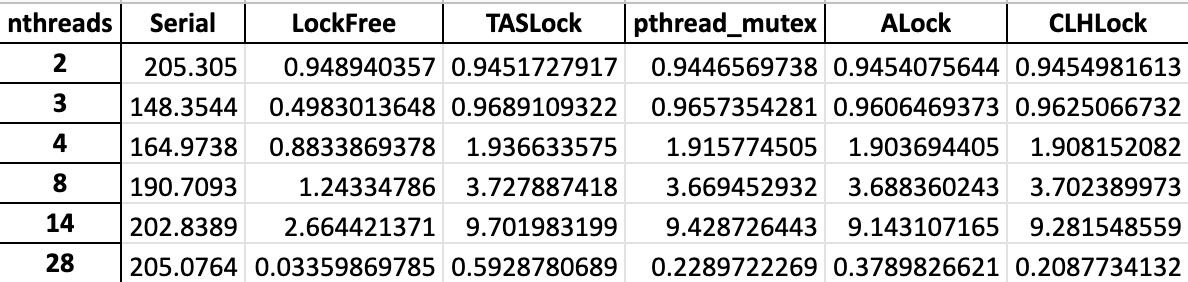
\includegraphics[width=\linewidth]{b_awe2000Data.png}\\ \null\\
\null\\
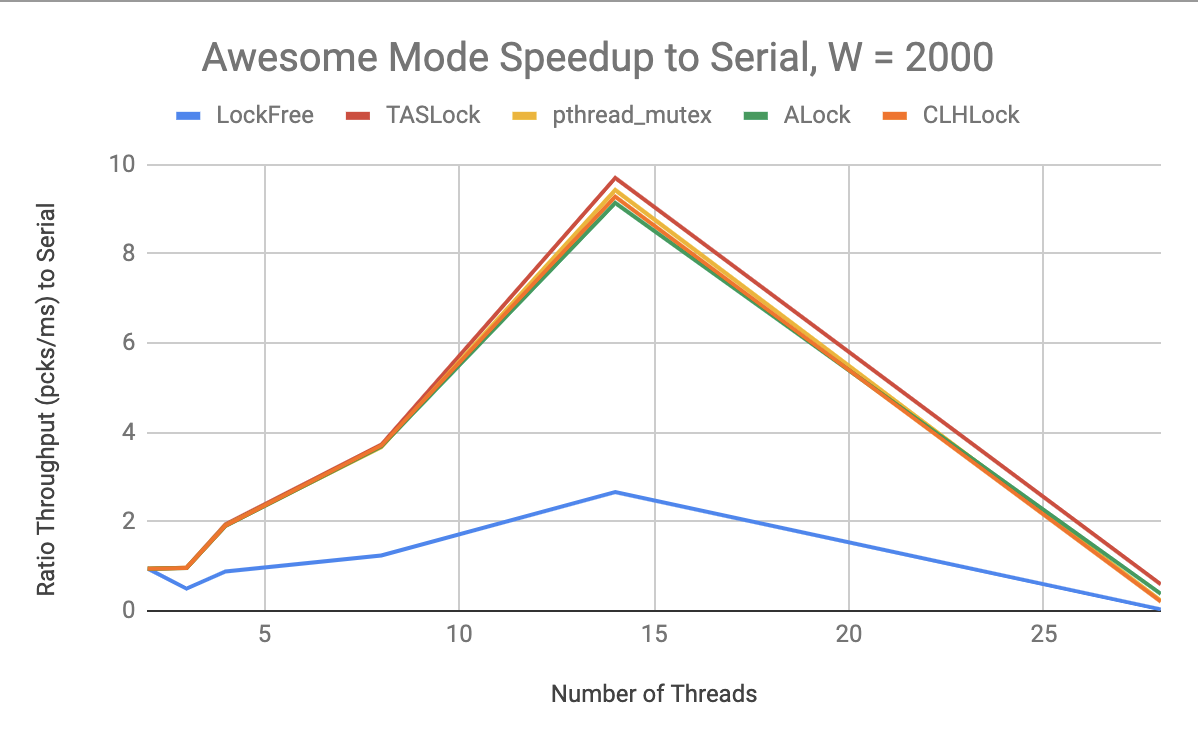
\includegraphics[width=\linewidth]{b_awe2000Graph.png}\\ \null\\
The jump in throughput from LockFree to Awesome grows even wider, with TASLock being $3.64\times$ faster than LockFree at 14 threads now. I expected this widening beforehand, as larger mean work leads to a large work variance between queues for exponential load and the other modes would cope much worse with this than Awesome.\\
TASLock has a higher absolute throughput ratio increase over CLHLock here than before - $(0.52 \times serial)$ pcks/ms at $W=2000$ versus $(0.25 \times serial)$ at $W=1000$. However, the ratios themselves have more than doubled from $W=1000$ to $W=2000$, so the relative throughput ratio increase of TASLock over CLHLock remains about the same.\\
\null\\Next are the data and graph for $W=4000$.\\
\null\\
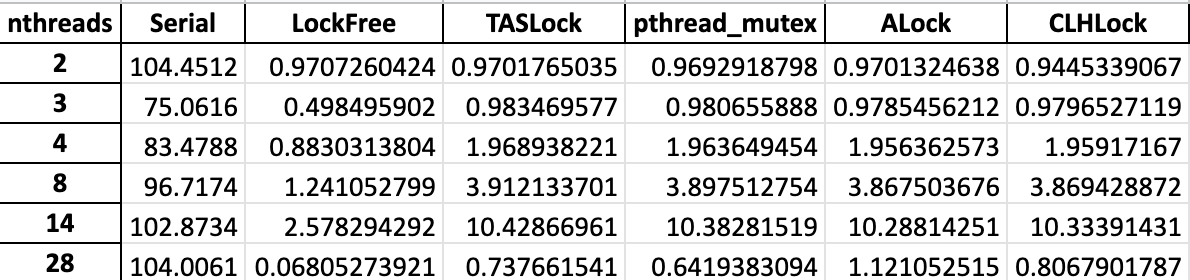
\includegraphics[width=\linewidth]{b_awe4000Data.png}\\ \null\\
\null\\
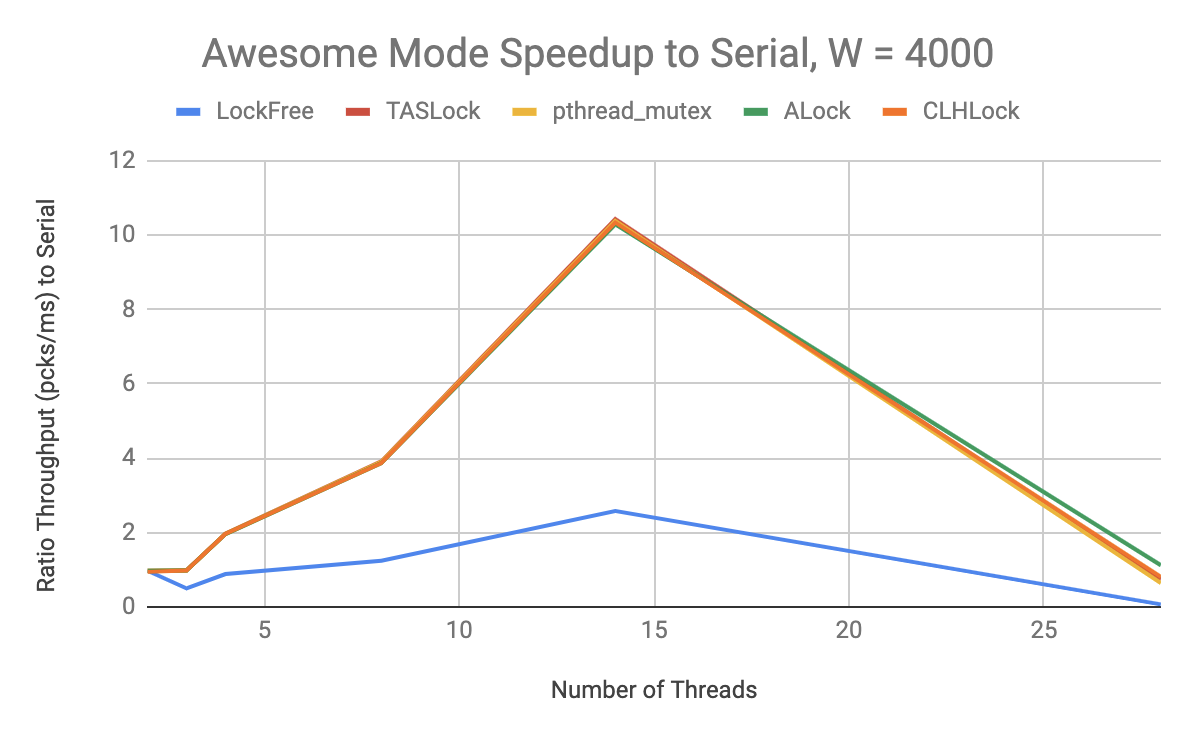
\includegraphics[width=\linewidth]{b_awe4000Graph.png}\\ \null\\
The ratio of Awesome to LockFree and to Serial is now about the same as it was at $W=4000$. This lack of additional relative speedup was not expected, but is likely because all threads are now being kept busy by the higher work, and there is no additional speed optimization via load balancing to be found.\\
The gap between locks is, as expected, now minimal.\\
\null\\Last for speedup data are the data and graph for $W=8000$.\\
\null\\
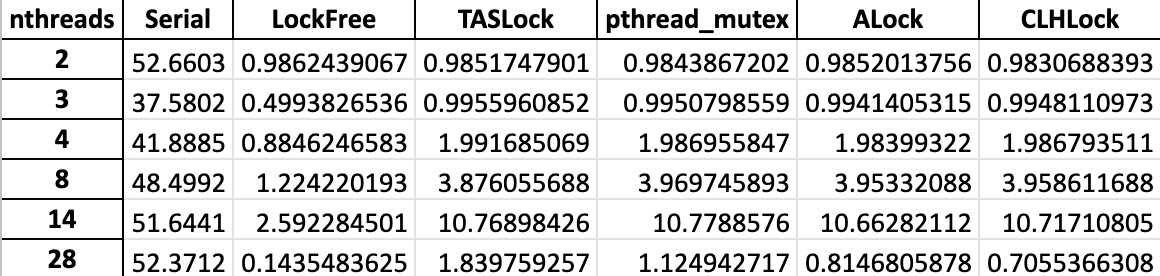
\includegraphics[width=\linewidth]{b_awe8000Data.png}\\ \null\\
\null\\
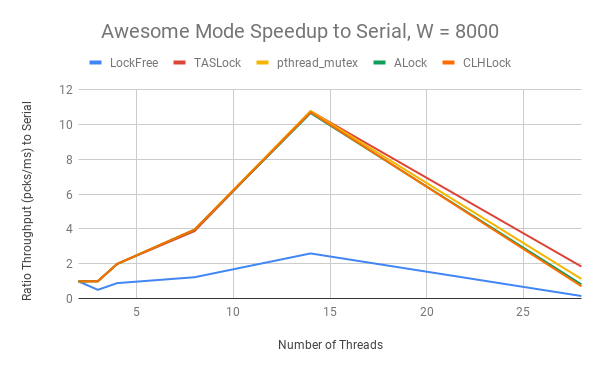
\includegraphics[width=\linewidth]{b_awe8000Graph.png}\\ \null\\
Following the observations from $W=4000$, the ratios remain about the same and locks are fairly indistinguishable.\\
Through all of these work levels, however, TASLock has remained faster than the queue-based locks. I edit the explanation I made at $W=1000$ to say that the locks most likely did not experience high enough contention at \textit{any} work level for the contention downsides of TASLock to outweigh the memory overhead of the queue-based locks.\\
\null\\I also thought it interesting to observe variances of single thread throughput, to demonstrate that Awesome truly does load balance significantly better than the one-thread-one-queue modes. Below is the variance of single thread throughput between LockFree and Awesome with all locks at the same numbers of threads taken before, taken at $W=8000$ to see maximal load balancing from Awesome.\\
\null\\
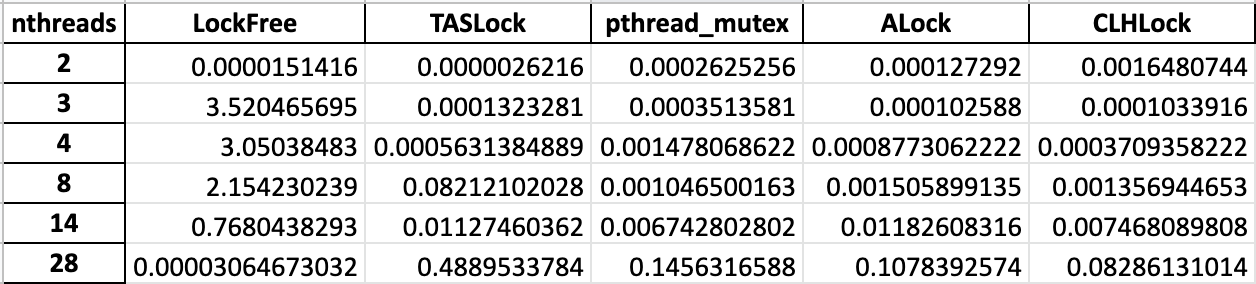
\includegraphics[width=\linewidth]{b_awefairData.png}\\ \null\\
\null\\
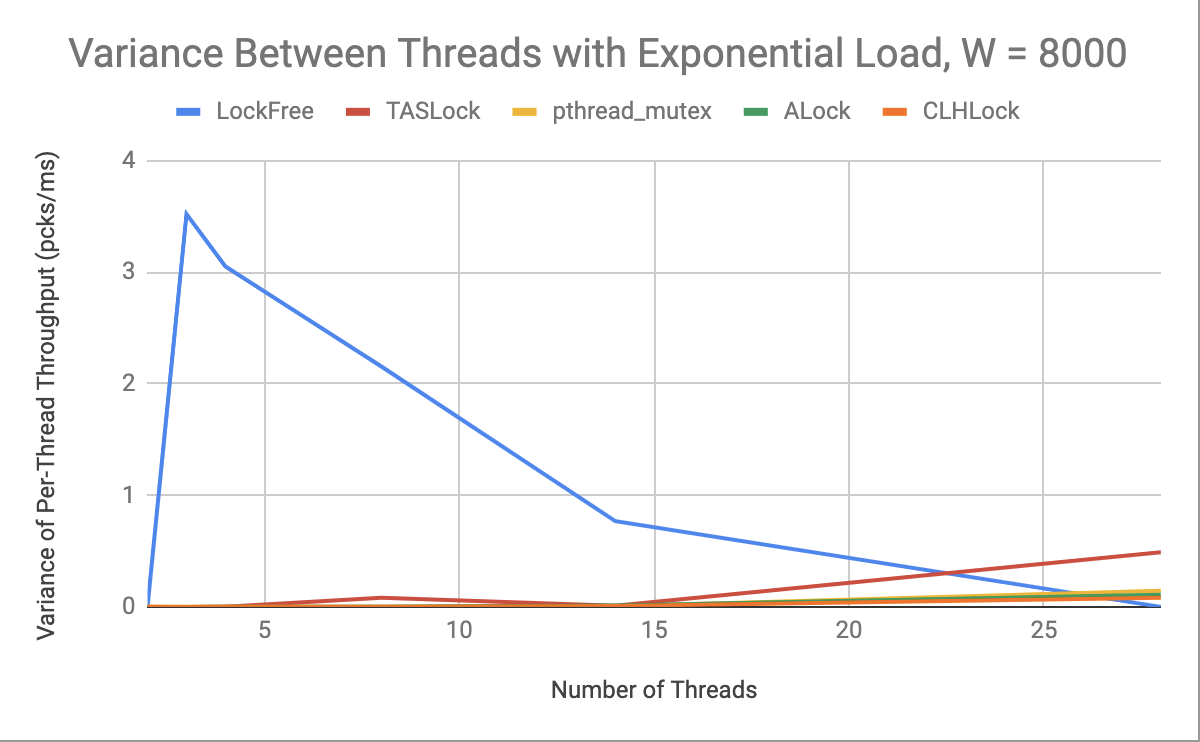
\includegraphics[width=\linewidth]{b_awefairGraph.png}\\ \null\\
As I expected, Awesome Mode with all locks maintained extremely low variance at all levels except 28 threads, which again can be forgiven due to context switching. The difference of variance between LockFree and Awesome is highest at the lowest amount of threads, and decreases as the number of threads increases. This is reasonable, because a higher amount of threads means proportionally less queues with high workload and proportionally less with low workload as well, giving LockFree some natural load balance that allows it to decrease variance.
\end{adjustwidth}
\end{document}
